%%%%%%%%%%%%%%%%%%%%%%%%%%%%%%%%%%%%%
% DB-KAPITEL
%%%%%%%%%%%%%%%%%%%%%%%%%%%%%%%%%%%%%
\chapter{Datenbankarchitektur und -entwicklung}
\renewcommand{\authorinitials}{MK}

\section{Einleitung}

Die Datenbank bildet das zentrale Fundament der Smart Shopping App, da sämtliche Produkt-, Listen- und Preisdaten effizient, sicher und flexibel gespeichert, abgerufen und miteinander verknüpft werden müssen. Die gewählte Architektur und das technologische Vorgehen haben maßgeblichen Einfluss auf Wartbarkeit, Erweiterbarkeit sowie die reibungslose Zusammenarbeit mit anderen Systemkomponenten – insbesondere bei modernen KI-gestützten Use Cases.

\section{Entwicklungsschritte und Migrationshintergrund}

Zu Projektbeginn wurde eine initiale, manuell aufgesetzte PostgreSQL-Datenbank bei Supabase verwendet. Supabase überzeugte durch eine schnelle Inbetriebnahme, webbasierte Oberfläche und REST-Schnittstellen, mit denen Entwickler sofort experimentieren konnten. Die Tabellen und Beziehungen wurden direkt im Supabase-Interface angelegt, was für den Proof-of-Concept und frühe Entwicklungsschritte ausreichend war.

Im Laufe des Projektes stiegen jedoch die Anforderungen: Mit wachsender Komplexität der Domäne, einer Vielzahl an Entitäten (Produkte, Varianten, Einkaufsliste, Angebote, Präferenzen usw.) und der Notwendigkeit häufiger Schemaänderungen zeigte sich, dass ein effizientes und modernes ORM-Framework notwendig ist. Die Wahl fiel auf den Einsatz von \textbf{Prisma} als ORM-Schicht, verbunden mit einer „klassischen“ PostgreSQL-Datenbank. Prisma erlaubt es, das Datenbankschema deklarativ in einer Versionierungsdatei (\texttt{schema.prisma}) zu pflegen, Migrationsprozesse sauber zu steuern und sämtliche Entitäten im Backend-Typen sicher und komfortabel zu verwalten.

\section{Gründe für die Migration auf Prisma \& klassische PostgreSQL-Instanz}

\begin{itemize}
    \item \textbf{Flexibilität und Wartbarkeit:} Schematische Änderungen – wie neue Felder, Tabellen, Relationen – können deklarativ vorgenommen und per Migration automatisch angewendet werden, ohne manuell Felder nachzupflegen.
    \item \textbf{Typisierung und Entwicklerfreundlichkeit:} Prisma generiert Typsicherungen und Methoden für alle Modelle, was bereits zur Entwicklungszeit Fehler reduziert und die Produktivität steigert.
    \item \textbf{Effizienz bei komplexen Entitäten:} Viele-zu-Viele- und verschachtelte Relationen (Produkte/Varianten, Kategorien, Präferenzen) werden elegant abgebildet und performant gemanagt.
    \item \textbf{KI-Integration:} Besonders für KI-Anwendungen ist es von Vorteil, das exakte Datenbankschema als Kontext bereitstellen zu können. Damit lassen sich automatisierte Abfragen, Generierung von Datenbankcode oder intelligente Schnittstellen viel einfacher umsetzen, da das Schema maschinenlesbar und selbstdokumentierend ist.
    \item \textbf{Teamwork und Automatisierbarkeit:} Dank Versionierung und automatischer Migration bleibt das Datenmodell im gesamten Team (und allen Umgebungen) konsistent.
\end{itemize}

\section{Struktur und Sinn der Datenbank für den Use Case}

Die folgende grafische Übersicht zeigt die wichtigsten Tabellen, Relationen und Primärschlüssel der finalen Datenbankstruktur, wie sie mit Prisma modelliert und als PostgreSQL-Datenbank betrieben wird:

% --- Bild/Diagramm einfügen ---
\begin{figure}[h!]
    \centering
    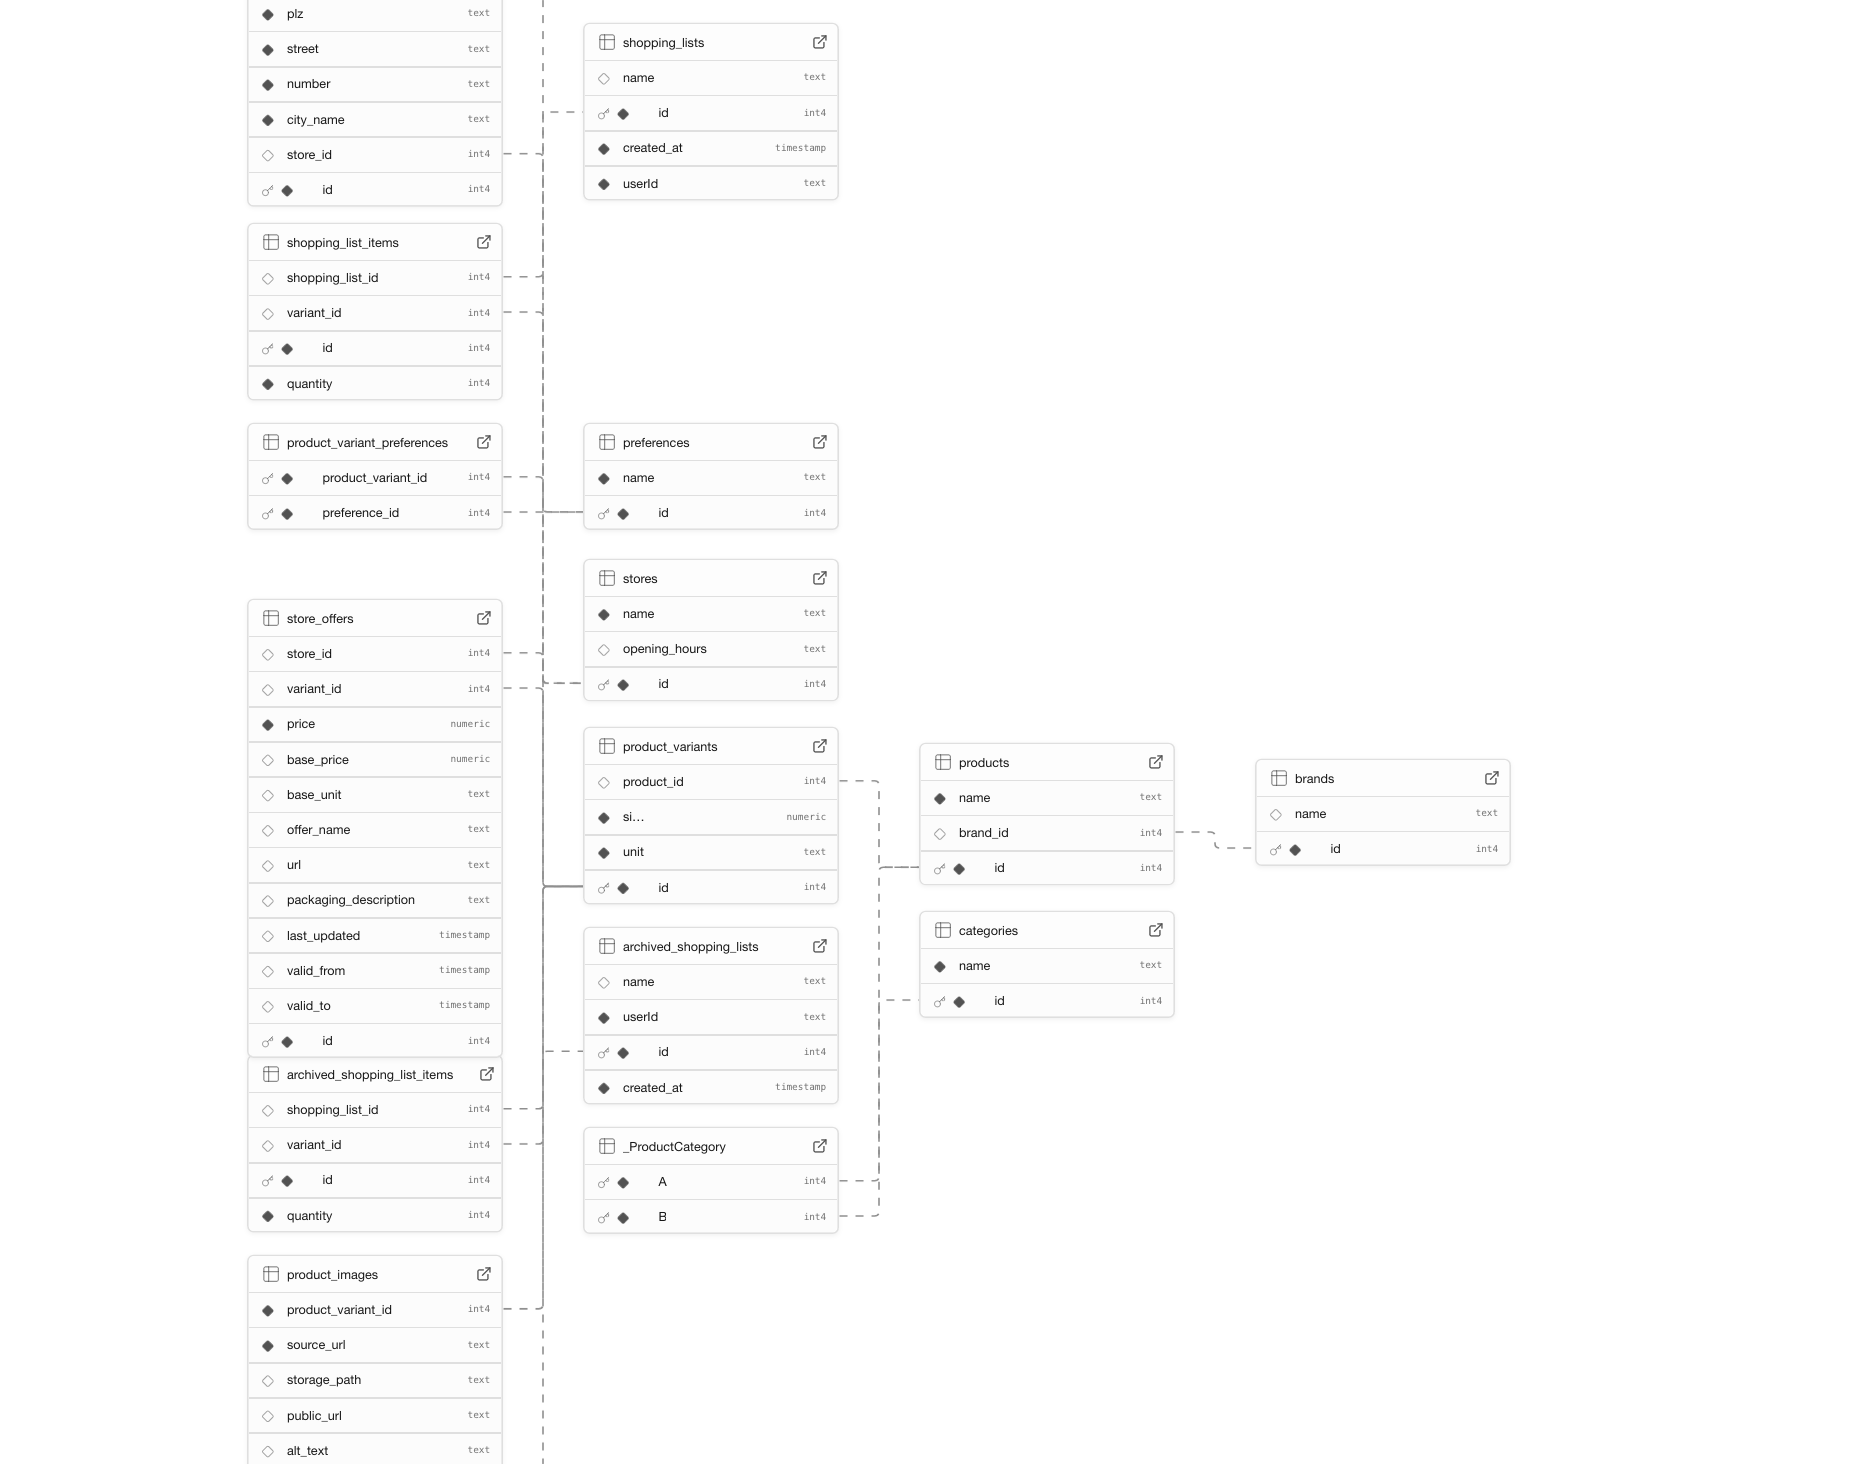
\includegraphics[width=0.98\textwidth]{media/supabase-schema-vgqtxqfvygduzmuwlmba.png}
    \caption{Schematische Übersicht der Projekt-Datenbank (als Supabase-Tabellenmodell)}
    \label{fig:db-schema}
\end{figure}

Die Datenbank vereint folgende Schlüsselaspekte unseres Use Cases:
\begin{itemize}
    \item \textbf{Produktspeicher:} Tabelle \texttt{products} enthält alle eindeutig erkannten Artikel (z.B. „Nutella 750g“), mit Zuordnung zur Marke, logischen Kategorien und beliebig vielen Varianten (\texttt{product\_variants} für Größen, Verpackungseinheiten etc.).
    \item \textbf{Marktübergreifender Vergleich:} Über \texttt{store\_offers} erhält jede Variante je Markt einen eigenen Preissatz – so kann die App tagesaktuell berechnen, welcher Supermarkt für die komplette Einkaufsliste der günstigste ist.
    \item \textbf{Einkaufslistenfunktion:} \texttt{shopping\_lists} und \texttt{shopping\_list\_items} Schnittstellen ermöglichen, nutzerbasierte Listen anzulegen und darin beliebige Produktvarianten in entsprechender Menge zu speichern. So bleibt die Architektur flexibel und beliebig skalierbar.
    \item \textbf{User-Zentrierung:} \texttt{UserId} bei Listen, Präferenzen (\texttt{preferences}), Favoriten, etc. koppelt alle Interaktionen eindeutig an das Anmelde-/Auth-System.
    \item \textbf{Angebots- und Preishistorie:} Über Felder wie \texttt{valid\_from}, \texttt{valid\_to} und \texttt{last\_updated} lassen sich jederzeit Angebotszeitpunkte oder Preisentwicklungen nachvollziehen.
    \item \textbf{Produktbilder und Metadaten:} Die Tabelle \texttt{product\_images} referenziert extern gespeicherte Bilder und bietet so für KI-basierte Such- oder Bilderkennungsideen einen klaren Ankerpunkt.
    \item \textbf{Erweiterbarkeit:} Zusätzliche Features (z.B. Präferenzen, Archiv, Benutzerfavoriten) können einfach durch weitere Tabellen oder Relationen ergänzt werden.
\end{itemize}

\section{Fazit}

Die konsequente Migration auf eine Prisma-verwaltete PostgreSQL-Datenbank erwies sich als zentraler Schritt zu einer robusten, flexiblen und wartungsfreundlichen Backend-Architektur. Für die Anforderungen einer KI-gestützten Smart Shopping App ist dieser Ansatz unverzichtbar: Das exakte, maschinenlesbare Datenmodell ist für Integration, automatisierte Weiterverarbeitung und Entwicklung innovativer Backend- bzw. KI-Features essenziell. Gleichzeitig garantiert die gewählte Architektur Zukunftssicherheit und einfache Erweiterbarkeit für neue Funktionen und Use Cases.

